\chapter[Publication 2]{Publication 2}

\section*{Light regime affects the seasonal cycle of Antarctic krill (\textit{Euphausia superba}): impacts on growth, feeding, lipid metabolism, and maturity}

Flavia Höring$^{1,2}$, Mathias Teschke$^{1}$, Lavinia Suberg$^{1}$, So Kawaguchi$^{3,4}$, and Bettina Meyer$^{1,2,5}$


{\scriptsize
1 Alfred Wegener Institute Helmholtz Centre for Polar and Marine Research, Section Polar Biological Oceanography, Am Handelshafen 12, 27570 Bremerhaven, Germany

2 Carl von Ossietzky University of Oldenburg, Institute for Chemistry and Biology of the Marine Environment (ICBM), Carl-von-Ossietzky-Str. 9-11, 26111 Oldenburg, Germany

3 Australian Antarctic Division, Department of the Environment and Energy, Channel Highway, Kingston, Tasmania 7050, Australia

4 Antarctic Climate and Ecosystems Cooperative Research Centre, University of Tasmania, Private Bag 80, Hobart, Tasmania 7001, Australia

5 Helmholtz Institute for Functional Marine Biodiversity (HIFMB) at the University of Oldenburg, 26111 Oldenburg, Germany 
}


Can. J. Zool. 96: 1203–1213 (2018) dx.doi.org/10.1139/cjz-2017-0353 

\section{Abstract}

Light regime is an important zeitgeber for Antarctic krill (\textit{Euphausia
superba} dana), which seems to entrain an endogenous timing system that
synchronizes its life cycle to the extreme light conditions in the Southern
Ocean. To understand the flexibility of Antarctic krill’s seasonal cycle, we
investigated its physiological and behavioural responses to different light
regimes and if an endogenous timing system was involved in the regulation of
these seasonal processes. We analysed growth, feeding, lipid content, and
maturity in a 2-year laboratory experiment simulating the latitudinal light
regimes at 52$^{\circ}$S and 66$^{\circ}$S and constant darkness under constant
food level. Our results showed that light regime affected seasonal cycles of
growth, feeding, lipid metabolism, and maturity in Antarctic krill. Seasonal
patterns of growth, feeding, and maturity persisted under constant darkness,
indicating the presence of an endogenous timing system. The maturity cycle
showed differences in critical photoperiods according to the simulated
latitudinal light regime. This suggests a flexible endogenous timing mechanism
in Antarctic krill, which may determine its response to future environmental
changes.

\section{Introduction}

Concerns are growing about the impact of global warming on the Antarctic marine
ecosystem. The observed changes in sea-ice extent and zooplankton distribution
may lead to trophic mismatches and thereby profound changes in the Southern
Ocean food web \citep{atkinson_long-term_2004, steinberg_long-term_2015}. To be
able to predict future changes, we need to better understand the adaptive
potential of polar key organisms such as the Antarctic krill (\textit{Euphausia
superba} Dana, 1850) \citep{meyer_seasonal_2010}.

Antarctic krill’s success in the Southern Ocean likely originates from its
ability to synchronize its life cycle to local photoperiod and food supply. It
has evolved seasonal patterns of growth, lipid turnover, metabolic activity
\citep{meyer_seasonal_2010}, and maturation \citep{kawaguchi_learning_2007}
that bring an evolutionary advantage to survive in an environment with strong
seasonal fluctuations of sea-ice extent, photoperiod, and primary production.
These seasonal patterns seem to vary according to latitudinal region, as it has
been observed that Antarctic krill near South Georgia (\SI{54}{\degree}S) had
lower lipid stores and higher feeding activities in winter compared with
regions at higher latitudes where near-constant darkness during winter limits
food supply \citep{schmidt_feeding_2014}. However, the mechanisms shaping these
seasonal rhythms remain poorly understood.

Photoperiod seems to play a major role in the modulation of the seasonal
rhythms of Antarctic krill. Laboratory experiments revealed that photoperiod
affected seasonal patterns of growth \citep{brown_temperature_2010}, maturity
\citep{hirano_antarctic_2003, teschke_effects_2008, brown_flexible_2011},
feeding, and metabolic activity \citep{teschke_simulated_2007}. It is not yet
clear if light regime also promotes acclimatization to the varying seasonal
conditions in different latitudinal habitats of Antarctic krill.

An endogenous timing system may be involved in the regulation of seasonal
rhy\-thms in Antarctic krill. Seasonal patterns of maturity were observed to
persist under constant darkness \citep{brown_flexible_2011}, indicating an
endogenous timing system that maintained the rhythm even if the zeitgeber
(environmental cue) was absent (= concept of a biological clock). Recent
studies suggest that Antarctic krill possesses a circadian clock that regulates
its daily metabolic output rhythms and is entrained by photoperiod
\citep{mazzotta_cry_2010, teschke_circadian_2011}. However, it is unknown if
the circadian clock is also involved in the timing of seasonal events in
Antarctic krill.

This study aims to investigate the effect of different light regimes on growth,
feeding, lipid metabolism, and maturity in Antarctic krill, as well as the
involvement of an endogenous timing system in the modulation of seasonal
rhythms. We analyse a unique data set from multiyear laboratory experiments
simulating different latitudinal light regimes (\SI{52}{\degree}S,
\SI{66}{\degree}S, constant darkness) and constant food supply over 2 years. We
will test (i) if light regime stimulates seasonal patterns of growth, feeding,
lipid metabolism, and maturity; (ii) if different latitudinal light regimes
cause different seasonal patterns; and (iii) if seasonal patterns persist under
constant darkness indicating an endogenous timing system.

\section{Materials and Methods}

\subsection{Antarctic krill collection and maintenance prior to the experiments}

Antarctic krill were caught with a rectangular mid-water trawl (RMT 8) on 12
February, 2013 (\SI{66}{\degree}\SI{47}{\arcmin}S,
\SI{65}{\degree}\SI{08}{\arcmin}E) during the voyage V3 12/13 of RSV Aurora
australis and on 15 January, 2015 (\SI{65}{\degree}\SI{31}{\arcmin}S,
\SI{141}{\degree}\SI{23}{\degree}E) during voyage V2 14/15. The sampling
methods are described in detail by \citet{king_krill_2003}. The sampled
Antarctic krill arrived at the Australian Antarctic Division aquarium in Hobart
on 22 February, 2013 and on 25 January, 2015, respectively. For acclimation and
for keeping of Antarctic krill until the start of the experiments, they were
transferred to \SI{800}{\liter} tanks (temperature \SI{0.5}{\celsius}) that
simulated the natural light regime at \SI{66}{\degree}S. A detailed description
of the Antarctic krill aquarium facility and the simulated light regime can be
found in \citet{kawaguchi_experimental_2010}.

\subsection{Photoperiodic-controlled laboratory experiments} 

Long-term laboratory experiments were conducted over a period of 2 years
starting in January 2015. Three different light regimes were tested, simulating
(1) natural light conditions at \SI{52}{\degree}S, (2) natural light conditions
at \SI{66}{\degree}S, and (3) constant darkness (DD) (Figs. \ref{Pub2_1}a,
\ref{Pub2_1}b). For each treatment, $250$ Antarctic krill were transferred from
the \SI{800}{\liter} acclimation tanks to a \SI{250}{\litre} experimental tank
connected to a recirculating chilled seawater system with a constant water
temperature of \SI{0.5}{\celsius}. For the initial experimental set-up,
Antarctic krill collected in 2013 were used (tanks A, B, E, F). 

%%%% Figure 1
\begin{figure}[ht!]
        \centering
        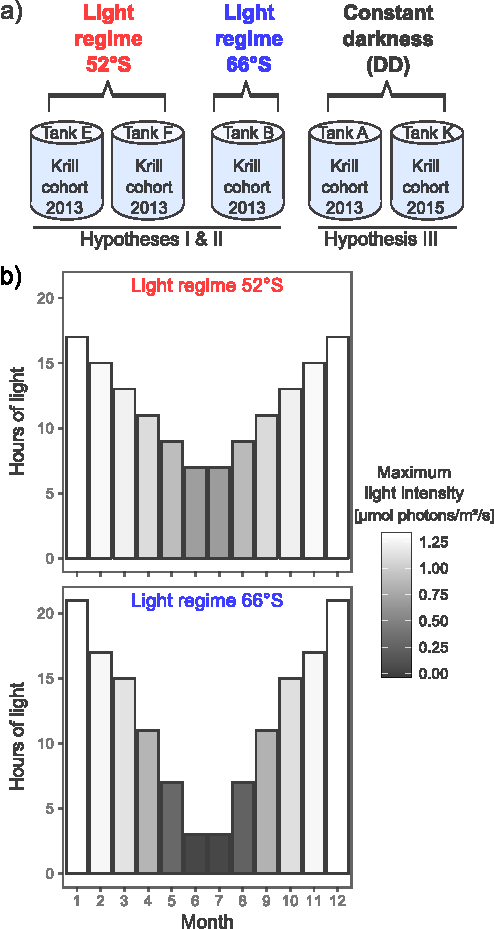
\includegraphics[height=10cm,keepaspectratio]{../Figures/Pub2_1.pdf}
        \caption{Long-term lab experiments at the Australian Antarctic Division: a) Experimental set-up and tested hypotheses, b) Simulated light regimes 55$^{\circ}$S and 66$^{\circ}$S.}
        \label{Pub2_1}
\end{figure}

However, due to increased mortality in tank A (treatment DD), an additional
tank for treatment DD (tank K) was set up in the beginning of March 2015 using
freshly caught Antarctic krill collected in 2015. The three different light
conditions were simulated within black lightproof plastic containers, one for
each experimental tank, using twin fluorescent tubes (Osram L18W/640 Cool
White) with a marine blue gel filter (Marine Blue 131; ARRI Australia Pty.
Ltd.). Light adjustment under treatments \SI{52}{\degree}S and
\SI{66}{\degree}S was carried out using a PC-controlled timer and dimming
system (\code{winDIM version 4.0e}; EEE, Portugal) with a maximum light
intensity of 100 lx (photon flux =
\SI{1.3}{\micro\mole\per\meter\square\per\second}) during midday in January
(corresponds to 1\% light penetration at \SI{30}{\meter} depth).  According to
the light regime, photoperiod and light-intensity profiles were adjusted at the
beginning of each month for each treatment. The simulated light-intensity
profiles for each treatment and month can be found in Supplementary Table S1.1 

The food level was held constant to remove that effect from our experiments
because we solely wanted to identify the effect that light regime had on the
seasonal cycle of Antarctic krill. Antarctic krill were fed daily between the
hours of 0830 and 0930 and the water flow in the tanks was turned off for
approximately 2 h to ensure feeding. The food comprised three live
laboratory-cultured algae (final concentrations were
\SI{1.5e4}{\cells\per\milli\liter} of \textit{Phaeodactylum tricornutum}
Bohlin, 1897, \SI{2e4}{\cells\per\milli\liter} of \textit{Geminigera cryophila}
(D.L. Taylor and C.C.  Lee) D.R.A. Hill, 1991,
\SI{2.2e4}{\cells\per\milli\liter} of \textit{Pyramimonas gelidicola} McFadden,
Moestrup and Wetherbee, 1982), three types of commercial algal paste
(\SI{1e4}{\cells\per\milli\liter} of \textit{Thalassiosira weissflogii}
(Grunow) G. Fryxell and Hasle, 1977 “TW 1200TM”,
\SI{5.1e4}{\cells\per\milli\liter} of Isochrysis Parke, 1949 “Iso 1800TM”,
\SI{4.8e4}{\cells\per\milli\liter} of Pavlova Butcher, 1952 “Pavlova 1800TM”;
Reed Mariculture, USA), and two types of prawn hatchery feeds (\SI{0.5}{\gram}
of FRiPPAK FRESH \#1CAR, \SI{0.5}{\gram} of FRiPPAK FRESH \#2CD; INVE,
Thailand).  Antarctic krill under treatment DD were fed in dim red light.
Moults and dead Antarctic krill were removed regularly from the tanks. 

Antarctic krill sampling of 6–10 individuals per tank and month was carried out
in the middle of each month during midday starting in February 2015 (for
treatment DD in dim red light). Due to different rates of mortality in the
tanks, the sampling scheme had to be adjusted during the course of the
experiment (Table \ref{Tab2_1}) to assure sampling over the whole experimental
period. Due to the problem with increased mortality under treatment DD
mentioned above, we decided to sample tanks A and K sequentially to ensure the
completion of the experiment over the 2-year period. 

% Please add the following required packages to your document preamble:
% \usepackage{booktabs}
\begin{table}[] \caption{Sampling scheme of the long-term experiment. Carapace
        length, digestive gland length and maturity score from these krill
        (\textit{E. superba}) were used for analysis of growth, feeding and
        maturity in this study. For lipid content analysis a reduced dataset
        was analysed.} 
        \label{Tab2_1}
{\scriptsize
\begin{tabular}{@{}llllllllll@{}}
\toprule
        \textbf{Treatment} & \textbf{Tank} & \textbf{Month 2-6} & \textbf{Month 7-13} & \textbf{Month 14-17} & \textbf{Month 18-19} & \textbf{Month 20-21} & \textbf{Month 22} & \textbf{Month 23} & \textbf{Month 24} \\ \midrule
52$^{\circ}$S      & E    & 10$\dagger$       & 6$\dagger$         & 6$\dagger$           & 6$\dagger$          &             & 8        &          &          \\
52$^{\circ}$S      & F    & 10        & 6          & 6            & 6           &             & 6        & 8        &          \\
66$^{\circ}$S      & B    & 10$\dagger$       & 6*$\dagger$        & 6$\dagger$           & 6$\dagger$          &             & 6        & 8        &          \\
DD        & A    & 10$\dagger$       & 6$\dagger$         & 6$\dagger$           &             &             &          &          &          \\
DD        & K    &           &            & 6            & 6$\dagger$          & 6           & 6        & 10       & 16       \\ \bottomrule
\end{tabular}
    \begin{tablenotes}
      \item Given numbers represent sampled individuals per month (n = 617).
      \item \textbf{*}: in July15 (month 7) one additional krill was sampled
      \item $\mathbf{\dagger}$: in April 15, July 15, October 15, January 16, April 16 and July 16 (months 4, 7, 10, 13, 16, 19) lipid content of 6 krill per month was analysed
     \end{tablenotes}

}
\end{table}


Live Antarctic krill was inspected under a stereomicroscope and the sex was
determined. Pictures of the carapace and the sexual organs (female thelycum and
male petasma) were taken with a Leica DFC 400 camera system (Leica
Microsystems, Germany). Carapace length (tip of the rostrum to posterior notch)
and digestive gland length (longest axis through carapace) were determined from
the pictures within the Leica \code{DFC Camera} software \code{version 7.7.1}
(Leica Microsystems, Switzerland). 

After visual inspection, the sampled Antarctic krill was immediately frozen in
liquid nitrogen. Frozen samples were stored at \SI{-80}{\celsius}.

The first inspection of the sex ratio within the experimental tanks revealed
that females dominated, with proportions of 71\%– 85\% per tank. 

\subsection{Growth analysis} 

Carapace length was used as a proxy for growth in the experiments. Antarctic
krill were sampled randomly from each experimental tank; thus, a general trend
observed in the carapace length data are assumed to display the general trend
of growth. 

The data analysis was performed in \code{RStudio version 1.0.136}
\citep{rstudio_team_rstudio:_2016}. Before the modelling process, a Pearson’s
product moment correlation was conducted to determine a potential difference in
growth pattern between male and female Antarctic krill; thus, the need for
separate models for each sex.  Due to the strong correlation (r = 0.82, p <
0.001) between males and females, based on the mean carapace length for each
sex across all treatments, data from both sexes were combined (n = 617). To
investigate the long-term trend (variable “time”) and the seasonal variability
(variable “month”) of Antarctic krill growth for each “treatment” (light
regime), a generalized additive mixed model (GAMM) with a Gaussian distribution
was used. An additive model was chosen over a linear one to resolve the
nonlinear relationship of the response and explanatory variables. The GAMM
takes the structure as specified by \citet{hastie_generalized_1987} and was
fitted using the gamm function in the mgcv package
\citep{wood_generalized_2006}. Random effects for “tank” were included in the
model to account for potential dependencies between individuals from the same
tank.  Prior to the modelling process, temporal autocorrelation was examined
using the acf function in \code{R}. Time series are often subject to
latitudinal dependencies between data points and not accounting for the
autocorrelation can result in biased estimates of model parameters
\citep{panigada_modelling_2008}. As autocorrelation was neither detected, nor
evident in residual analysis during model validation, no temporal
autocorrelation term was included in the final model. 

Smoothed terms were fitted as regression splines (variable “time”), apart for
the variable “month”, which was modelled using cyclic cubic regression splines,
setting knots manually between 1 (January) and 12 (December) to account for the
circular nature of this term. Differences in temporal pattern between the three
light regimes (\SI{52}{\degree}S, \SI{66}{\degree}S, DD) were implemented using
the by- argument of the gamm function, which allows for the creation of
separate smoothers for each level of the treatment factor (light regime) over
the temporal variables “month” and “time”. Hence, separate parameter estimates
for the temporal variables are obtained for each treatment level. To avoid
overfitting, the smooth function of the variable “month” was manually
restricted to k = 5. Model selection was conducted using manual
stepwise-backward selection based on Akaike’s information criterion (AIC)
\citep{akaike_likelihood_1981}. If the addition of a term led to an AIC
decrease of >2 per degree of freedom, or an increase of the adjusted R2, or if
the term was significant, then the term was included in the model. Model fit
was examined by residual analysis.

\subsection{Feeding Analysis}

The feeding index (\%) was calculated as digestive gland length $\times$
(carapace length)-1 $\times$ 100. Data of males and females were combined
because of the strong correlation of monthly mean values (Pearson’s product
moment correlation, r = 0.95, p < 0.001). To investigate a temporal pattern in
the feeding index of Antarctic krill for each treatment, a GAMM was employed as
described above (section Growth analysis). The smooth function of the variable
“time” was manually restricted to k = 6.

\subsection{Lipid content analysis}

Every 3 months from April 2015 to July 2016, six replicate samples from each
treatment were tested for their lipid content. Lipids were extracted from the
carapace, which was separated from the frozen samples with a scalpel on dry ice
prior to extraction. Lipid extraction was performed with
dichloromethane:methanol (2:1, v:v) according to the method described by
\citet{hagen_lipids_2000}. Lipid content was determined gravimetrically and was
calculated in percentage of dry mass. One data point (sample code “Jan16\_E04”)
was removed due to the negative value of lipid content that indicated incorrect
measurement for that individual. 

Lipid content differed between male and female Antarctic krill (Pearson’s
product moment correlation of pooled monthly mean values, r = 0.26, p = 0.62);
therefore, statistical analysis was performed separately for each sex. Data for
males were not sufficient for robust modelling and only females were considered
for this analysis (n = 83). Only one tank for each time point and treatment was
available, therefore a mixed model to resolve a potential tank effect could not
be employed. For treatment DD, five samples were available from a second tank,
but these were not sufficient for the inclusion of a random effect. Therefore,
a generalized additive model (GAM) was employed to examine the temporal pattern
of female Antarctic krill lipid content, following the protocol described in
section Growth analysis. The smooth function of the variable “time” was
manually restricted to k = 6. Because the variable “month” was not significant,
it was excluded from the final model.

\subsection{Maturity Analysis}

The maturity stage of the sampled Antarctic krill was assessed by analysing
pictures of the external sexual organs according to \citet{makarov_stages_1980}
and \citet{thomas_thelycum_1987}. A maturity score was assigned using the
method of \citet{brown_temperature_2010, brown_flexible_2011}. Due to the
ordinal characteristic of the maturity scores, Pearson correlation of monthly
mean values could not be per- formed with the data set. Therefore, we visually
inspected the relationship between maturity score and hours of light in males
and females. Seasonal maturity scores differed between male and female
Antarctic krill (Fig. \ref{Pub2_2}); therefore, statistical analysis was
performed on females only (n = 493), as there were not sufficient data to allow
for modelling males separately. To investigate the temporal pattern of maturity
of female Antarctic krill for each treatment, a GAMM was employed as described
in section Growth analysis. Because model residuals were autocorrelated, an
auto-regressive correlation structure of the order 1 was added, which improved
model fit and resolved the dependencies between residuals. Maturity scores are
represented as whole numbers and take values between 3 and 5. Therefore, the
GAMM was initially modelled using a Poisson distribution with a logarithmic
link function between predictor and response. Due to overdispersion, a negative
binomial GAMM had to be used. The smooth function of the variable “time” was
manually restricted to k = 6. 

%%%%%%%% Figure 2
\begin{wrapfigure}{O}{0.4\textwidth}
       \vspace{-20pt}
        \centering
        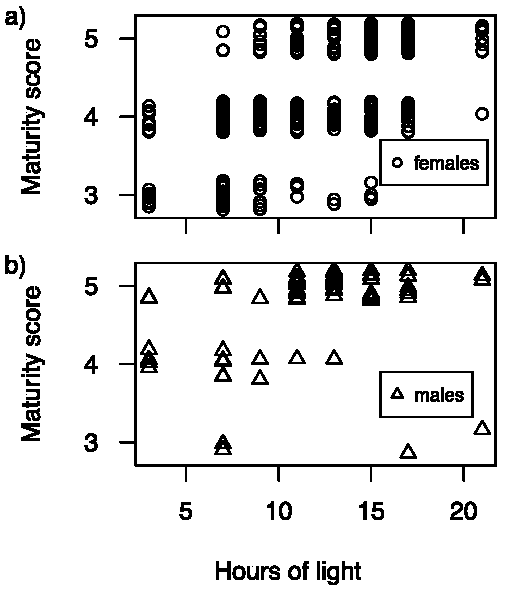
\includegraphics[width=0.35\textwidth]{../Figures/Pub2_2.pdf}
        \vspace{-15pt}
        \caption{Relationship between maturity score and hours of light in a)
        females and b) males.}
        \label{Pub2_2}
         \vspace{-10pt}
\end{wrapfigure}

To examine differences in the critical photoperiod between latitudinal light
regimes 52$^{\circ}$S and 66$^{\circ}$S, a logistic regression was used. As
only full maturity was investigated, maturity scores <5 were set to zero and
full maturity (score = 5) was set to one in all samples, resulting in a data
set of zeros and ones. The relationship between full maturity of female
Antarctic krill and photoperiod was modelled with a binomial generalized linear
mixed model (GLMM) with a logit function between predictor and response and an
interaction term for factor “treatment” and continuous variable “hours of
light”. The model was fitted using the glmer function from the lme4 library. To
account for dependencies between individuals from the same tank, random effects
for “tank” were included in the model. Model fit was assessed by constructing a
receiver operating characteristic (ROC) curve using the pROC package in R,
where the area under the curve (AUC) indicates the goodness of fit
\citep{boyce_evaluating_2002}. Values below 0.7 are considered poor and 1.0
represents a perfect fit \citep{cumming_using_2000}. The critical photoperiod
(= photoperiod, when the probability to be fully mature is 50\%) was predicted
from the 95\% confidence intervals.

\subsection{Data archiving} 

Processed data have been uploaded to the database PANGAEA and can be accessed
under \url{https://doi.pangaea.de/10.1594/PANGAEA.885889.}

\section{Results}

\subsection{Growth Analysis} 

Carapace length ranged from 8.1 to 19.02 mm with a mean ($\pm$SD) of 11.71 mm
($\pm$1.61 mm) across the whole data set. The GAMM (model M1; Table
\ref{Tab2_2}) revealed significant seasonal and interannual patterns in growth,
which were similar across all treatments (Figs. \ref{Pub2_3}a, \ref{Pub2_3}b).
Shrinkage was observed in the beginning of the experiments. A significant
seasonal variability with shrinkage towards austral winter (June to August) and
growth towards austral summer (December to February) was observed under
treatments 52$^{\circ}$S and DD (not significant under treatment
66$^{\circ}$S).

%%%%%%%% Figure 3
\begin{figure}[ht!]
        \centering
        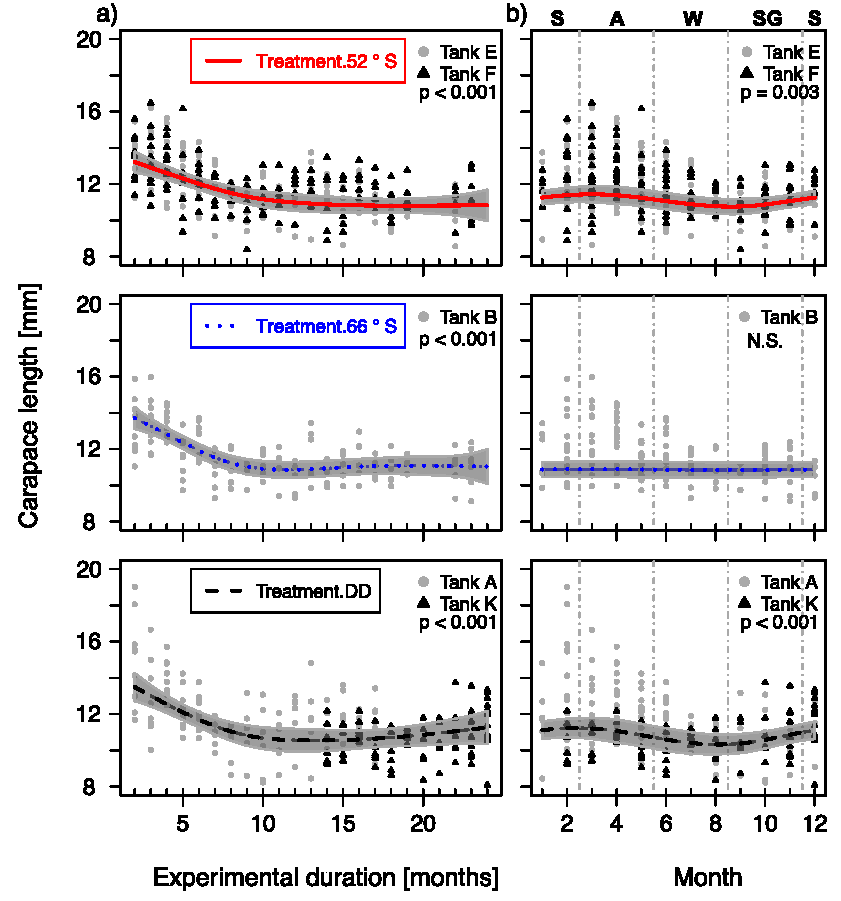
\includegraphics[width=0.85\textwidth]{../Figures/Pub2_3.pdf}
        \caption{Estimated smooth terms of the GAMM for carapace length within
        treatments 52$^{\circ}$S, 66$^{\circ}$S and DD with a) explanatory
        variable time (thin plate regression spline smooth term) showing the
        general trend over the whole experimental period and b) explanatory
        variable month (cyclic smooth term) representing the seasonal trend
        over the months of the year. The smoothers (lines) are displayed with
        95\% confidence intervals (shading), the raw data points for
        experimental tanks (shapes) and the p-value. The seasonal periods are
        indicated by vertical dashed lines and the following abbreviations: SG
        - spring, S - summer, A - autumn, W - winter.}
        \label{Pub2_3}
\end{figure}

\begin{table}[]
\centering
{\scriptsize
\caption{Model results, showing model statistics for parametric coefficients (estimates, standard errors (SD), \textit{z}- or \textit{t}-values and \textit{p}-values), a measure of explained variance of the model (Deviance or Adjusted $R^{2}$ (Adj. $R^{2}$)) and non-parametric terms where applicable (estimated degrees of freedom (edf), \textit{F}-statistic and \textit{p}-values). }
\label{Tab2_2}
\begin{tabular}{@{}lllllll@{}}
\toprule \\
\textbf{Intercept} & \textbf{Estimate} & \textbf{SD} & \textbf{\textit{t}-value} & \textbf{\textit{p}-value} & \textbf{Adj. R}$\mathbf{^{2}}$ & \\
\textbf{M1} & $11.67$ & $0.12$ & $101$ & $<0.001$ & $0.39$ & \\
\midrule
& \multicolumn{2}{c}{Treatment 52$^{\circ}$S} & \multicolumn{2}{c}{Treatment 66$^{\circ}$S} & \multicolumn{2}{c}{Treatment DD} \\
% M1 Test
\textbf{Variable} & \cellcolor{gray!50}\textbf{Time} & \cellcolor{gray!50}\textbf{Month} &\cellcolor{blue!25}\textbf{Time} & \cellcolor{blue!25}\textbf{Month} & \cellcolor{blue!50}\textbf{Time} & \cellcolor{blue!50}\textbf{Month} \\

\textbf{Smooth (edf)} & \cellcolor{gray!50}2.84 & \cellcolor{gray!50}1.74 &\cellcolor{blue!25}3.56 & \cellcolor{blue!25}0.39 & \cellcolor{blue!50}3.32 & \cellcolor{blue!50}1.8 \\

\textbf{F-value} & \cellcolor{gray!50}32.8 & \cellcolor{gray!50}1.95 &\cellcolor{blue!25}20.65 & \cellcolor{blue!25}0.15 & \cellcolor{blue!50}20.31 & \cellcolor{blue!50}2.46 \\

\textbf{p-value} & \cellcolor{gray!50}<0.001 & \cellcolor{gray!50}0.003 &\cellcolor{blue!25}<0.001 & \cellcolor{blue!25}0.13 & \cellcolor{blue!50}<0.001 & \cellcolor{blue!50}<0.001 \\

\midrule
% M2 Test
\textbf{Intercept} & \textbf{Estimate} & \textbf{SD} & \textbf{\textit{t}-value} & \textbf{\textit{p}-value} & \textbf{Adj. R}$\mathbf{^{2}}$ & \\
\textbf{M2} & $42.08$ & $0.22$ & $189.8$ & $<0.001$ & $0.64$ & \\
\midrule

\textbf{Variable} & \cellcolor{gray!50}\textbf{Time} & \cellcolor{gray!50}\textbf{Month} &\cellcolor{blue!25}\textbf{Time} & \cellcolor{blue!25}\textbf{Month} & \cellcolor{blue!50}\textbf{Time} & \cellcolor{blue!50}\textbf{Month} \\

\textbf{Smooth (edf)} & \cellcolor{gray!50}2.87 & \cellcolor{gray!50}5.09 &\cellcolor{blue!25}2.55 & \cellcolor{blue!25}1.47 & \cellcolor{blue!50}3.13 & \cellcolor{blue!50}2.79 \\

\textbf{F-value} & \cellcolor{gray!50}41.42 & \cellcolor{gray!50}4.2 &\cellcolor{blue!25}92.84 & \cellcolor{blue!25}0.39 & \cellcolor{blue!50}64.52 & \cellcolor{blue!50}1.4 \\

\textbf{p-value} & \cellcolor{gray!50}<0.001 & \cellcolor{gray!50}<0.001 &\cellcolor{blue!25}<0.001 & \cellcolor{blue!25}0.041 & \cellcolor{blue!50}<0.001 & \cellcolor{blue!50}<0.001 \\
\midrule
% M3 Test
\textbf{Intercept} & \textbf{Estimate} & \textbf{SD} & \textbf{\textit{t}-value} & \textbf{\textit{p}-value} & \textbf{Deviance} & \\
\textbf{M3} & $17.21$ & $0.77$ & $22.33$ & $<0.001$ & $50.9\%$ & \\
\midrule

\textbf{Variable} & \cellcolor{gray!50}\textbf{Time} & \cellcolor{gray!50} &\cellcolor{blue!25}\textbf{Time} & \cellcolor{blue!25} & \cellcolor{blue!50}\textbf{Time} & \cellcolor{blue!50} \\

\textbf{Smooth (edf)} & \cellcolor{gray!50}3.58 & \cellcolor{gray!50} &\cellcolor{blue!25}3.82 & \cellcolor{blue!25} & \cellcolor{blue!50}1.0 & \cellcolor{blue!50} \\

\textbf{F-value} & \cellcolor{gray!50}1.16 & \cellcolor{gray!50} &\cellcolor{blue!25}14.97 & \cellcolor{blue!25} & \cellcolor{blue!50}0.05 & \cellcolor{blue!50} \\

\textbf{p-value} & \cellcolor{gray!50}0.3 & \cellcolor{gray!50} &\cellcolor{blue!25}<0.001 & \cellcolor{blue!25} & \cellcolor{blue!50}0.82 & \cellcolor{blue!50} \\
\midrule

% M4 Test
\textbf{Intercept} & \textbf{Estimate} & \textbf{SD} & \textbf{\textit{t}-value} & \textbf{\textit{p}-value} &  \textbf{Adj. R}$\mathbf{^{2}}$ & \\
\textbf{M4} & $1.43$ & $0.01$ & $134.9$ & $<0.001$ & $0.45$ & \\
\midrule

\textbf{Variable} & \cellcolor{gray!50}\textbf{Time} & \cellcolor{gray!50}\textbf{Month} &\cellcolor{blue!25}\textbf{Time} & \cellcolor{blue!25}\textbf{Month} & \cellcolor{blue!50}\textbf{Time} & \cellcolor{blue!50}\textbf{Month} \\

\textbf{Smooth (edf)} & \cellcolor{gray!50}1.0 & \cellcolor{gray!50}4.14 &\cellcolor{blue!25}1.88 & \cellcolor{blue!25}4.07 & \cellcolor{blue!50}3.33 & \cellcolor{blue!50}2.88 \\

\textbf{F-value} & \cellcolor{gray!50}6.1 & \cellcolor{gray!50}15.0 &\cellcolor{blue!25}5.84 & \cellcolor{blue!25}7.7 & \cellcolor{blue!50}4.58 & \cellcolor{blue!50}1.19 \\

\textbf{p-value} & \cellcolor{gray!50}0.014 & \cellcolor{gray!50}<0.001 &\cellcolor{blue!25}0.002 & \cellcolor{blue!25}<0.001 & \cellcolor{blue!50}0.04 & \cellcolor{blue!50}<0.001 \\
\midrule
\textbf{M5} & \textbf{Estimate} & \textbf{SD} & \textbf{\textit{z}-value} & \textbf{\textit{p}-value} &  \textbf{AUC} & \\
\textbf{Intercept} & $-6.09$ & $0.78$ & $-7.86$ & $<0.001$ & $0.77$ & \\
\textbf{Hours of Light} & $0.49$ & $0.06$ & $7.86$ & $<0.001$ & & \\
\textbf{Treatment} & $1.22$ & $1.25$ & $0.98$ & $0.4$ & & \\
\textbf{Interaction: Light * Latitude} & $-0.16$ & $0.09$ & $-1.73$ & $0.084$ & & \\

\bottomrule
\end{tabular}
    \begin{tablenotes}
      \item Significant \textit{p}-values of explanatory variables are in bold.
      \item \textbf{M1}: GAMM for carapace length over time for each treatment with random effects for tank
      \item \textbf{M2}: GAMM for feeding index over time for each treatment and random effects for tank
      \item \textbf{M3}: GAM for lipid content of females over time for each treatment 
      \item \textbf{M4}: Negative binomial GAMM for female maturity over time for each treatment with random effects for tank and AR1-correlation structure
      \item \textbf{M5}: Binomial GLMM for full maturity of females in relation to hours of light with interaction term for treatment (52$^{\circ}$S and 66$^{\circ}$S) and random effects for tank effect, AUC = ‘Area under the curve’ from ROC-curve analysis serves as an indication of model fit
    \end{tablenotes}
}
\end{table}


\subsection{Feeding}

The feeding index data ranged from 25.15\% to 66.09\% with a mean ($\pm$SD) of
42.00\% ($\pm$6.58\%). 

The GAMM revealed significant changes in the feeding index over time (model M2;
Table 2). We observed an increase of the feeding index throughout the
experimental period in all treat- ments and a final stagnation in treatments
52$^{\circ}$S and DD (Figs. \ref{Pub2_4}a, \ref{Pub2_4}b). The seasonal trend
differed between treatments. In treatment 52$^{\circ}$S, the feeding index
strongly increased during the autumn period (March to May) with a subsequent
decrease and stabilization during the rest of the year. The seasonal trend in
treatment 66$^{\circ}$S was very weak and will therefore not be described
further. In treatment DD, the feeding index increased over a longer period
(March to July) and decreased during the rest of the year.

%%%%%%%%%% Figure 4
\begin{figure}[htb!]
        \centering
        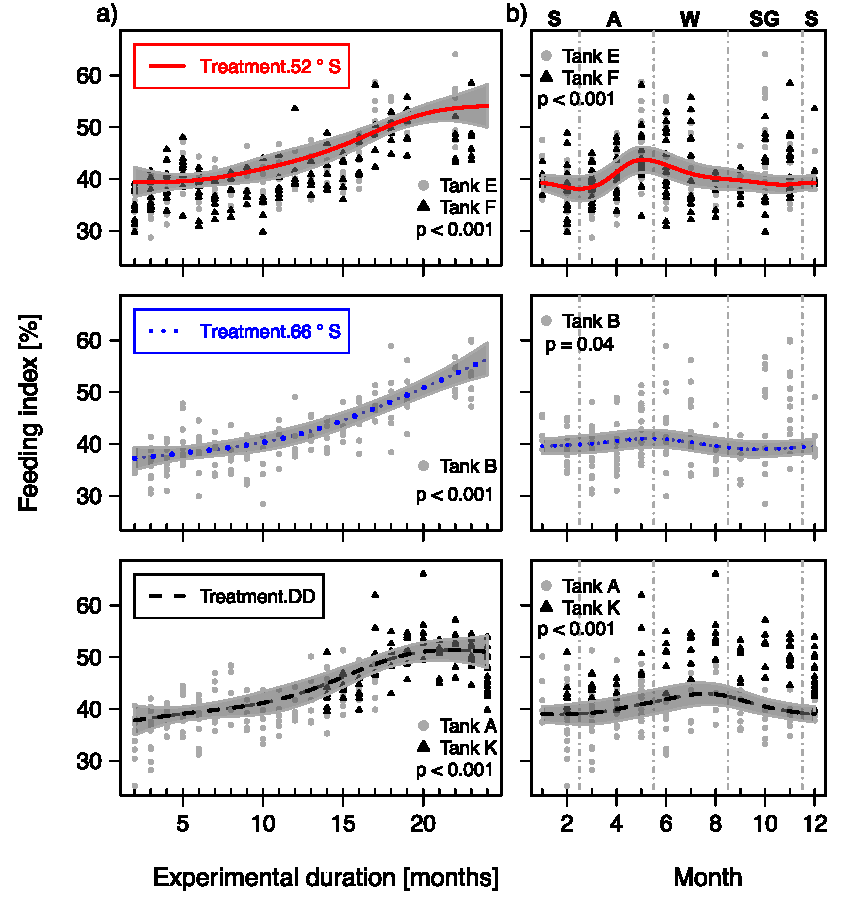
\includegraphics[width=0.85\textwidth]{../Figures/Pub2_4.pdf}
        \caption{Estimated smooth terms of the GAMM for feeding index within
        treatments 52$^{\circ}$S, 66$^{\circ}$S and DD with a) explanatory
        variable time (thin plate regression spline smooth term) showing the
        general trend over the whole experimental period and b) explanatory
        variable month (cyclic smooth term) representing the seasonal trend
        over the months of the year. The smoothers (lines) are displayed with
        95\% confidence intervals (shading), the raw data points for
        experimental tanks (shapes) and the p-value. The seasonal periods are
        indicated by vertical dashed lines and the following abbreviations: SG
        - spring, S - summer, A - autumn, W - winter.}
        \label{Pub2_4}
\end{figure}

%%%%%%%%%%% Figure 5
\begin{figure}
        \centering
        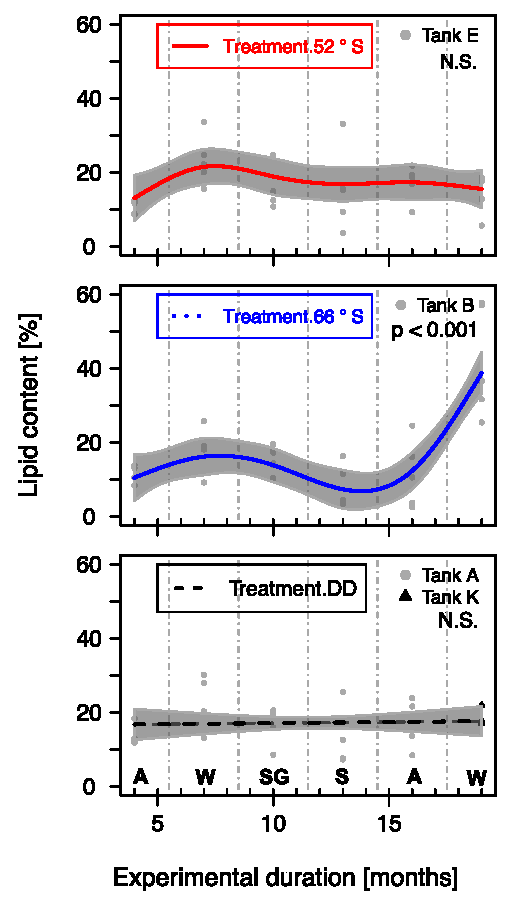
\includegraphics[width=0.75\textwidth]{../Figures/Pub2_5.pdf}
        \caption{Estimated smooth terms of the GAM for lipid content in females
        within treatments 52$^{\circ}$S, 66$^{\circ}$S and DD. The explanatory
        variable time (thin plate regression spline smooth term) is showing the
        general trend over the whole experimental period. The smoothers (lines)
        are displayed with 95\% confidence intervals (shading), the raw data
        points for experimental tanks (shapes) and the p-value. The seasonal
        periods are indicated by vertical dashed lines and the following
        abbreviations: SG - spring, S - summer, A - autumn, W - winter.}
        \label{Pub2_5}
\end{figure}

\subsection{Lipids}

The lipid content data of males and females ranged from 2.53\% to 57.75\% with
a mean ($\pm$SD) of 17.04\% ($\pm$9.12\%). The GAM considering female lipid
content data only (model M3; Table 2) revealed significant differences in
temporal variability of lipid content be- tween the experimental treatments
(Fig. \ref{Pub2_5}). Even though the variable “month” was not significant, a
resembling seasonal pattern was observed in the interannual trend under
treatment 66$^{\circ}$S with an increase towards austral winter and a decrease
towards austral summer. The increase of lipid content during the second winter
was much stronger than the first winter. No significant patterns were found for
treatments 52$^{\circ}$S and DD.

\subsection{Maturity}

Implementing the negative binomial GAMM for female maturity (model M4; Table
2), we found a significant seasonal cycle of maturity under treatments
52$^{\circ}$S, 66$^{\circ}$S, and DD with sexual regression towards austral
winter and sexual re-maturation towards austral spring and summer (Figs.
\ref{Pub2_6}a, \ref{Pub2_6}b). Significant interannual patterns differed
between treatments. In treatments 52$^{\circ}$S and 66$^{\circ}$S, a slight
decrease of maturity over the whole study period was observed. The interannual
pattern in treatment DD showed that sexual regression was only completed during
the first winter of the experiments. 


%%%%%%%%%%% Figure 6
\begin{figure}
        \centering
        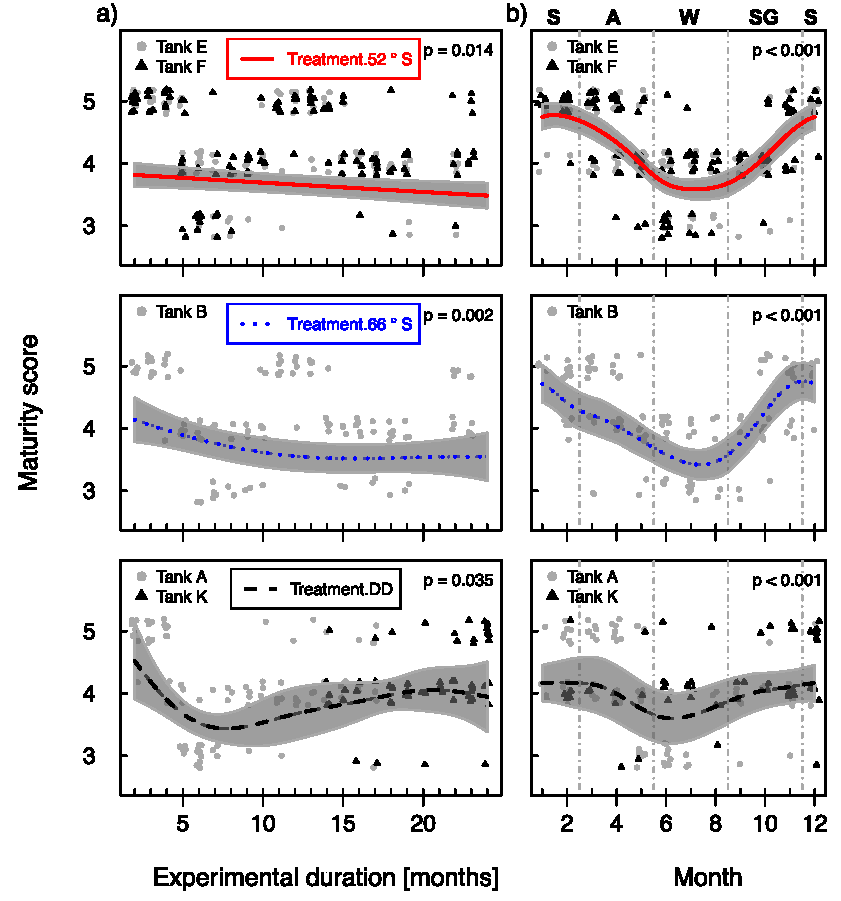
\includegraphics[width=0.85\textwidth]{../Figures/Pub2_6.pdf}
        \caption{Estimated smooth terms of negative binomial GAMM for female
        maturity within treatments 52$^{\circ}$, 66$^{\circ}$S and DD with a)
        explanatory variable time (thin plate regression spline smooth term)
        showing the general trend over the whole experimental period and b)
        explanatory variable month (cyclic smooth term) representing the
        seasonal trend over the months of the year. The smoothers (lines) are
        displayed with 95\% confidence intervals (shading), the jittered raw
        data points for experimental tanks (shapes) and the p-value. The
        seasonal periods are indicated by vertical dashed lines and the
        following abbreviations: SG - spring, S - summer, A - autumn, W -
        winter.}
        \label{Pub2_6}
\end{figure}

The binomial GLMM (model M5; Table 2) suggests that the variable “hours of
light” significantly affects female maturity in treatments 52$^{\circ}$S and
66$^{\circ}$S. The interaction term between “hours of light” and “treatment”
was marginally not significant. When investigating the critical photoperiod at
the probability of 50\%, differences between the treatments were found (Fig.
\ref{Pub2_7}). For treatment 52$^{\circ}$S, the critical photoperiod was
estimated as 12.5 h of light with 95\% confidence intervals (11.86, 13.22). For
treatment 66$^{\circ}$S, an estimate of 14.76 h of light with 95\% confidence
intervals (13.3, 16.3) was found.


%%%%%%%%%%% Figure 7

\begin{wrapfigure}{O}{6cm}
        \centering
        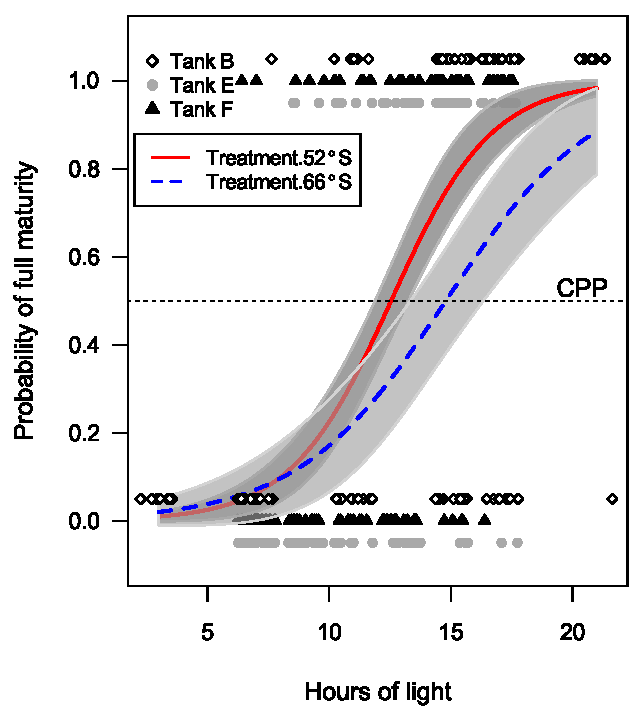
\includegraphics[height=7cm, keepaspectratio]{../Figures/Pub2_7.pdf}
        \caption{Results from the logistic regressions for 52$^{\circ}$S and
        66$^{\circ}$S: Estimated trends of the binomial GLMM (lines) are shown
        with 95\% confidence intervals (shading) and jittered raw data points
        for experimental tanks (shapes). The horizontal line indicates the 50\%
        probability level for the critical photoperiod (CPP).}
        \label{Pub2_7}
\end{wrapfigure}

\section{Discussion}

We present findings from the first 2-year laboratory experiments investigating
the effect of light regime and the biological clock on the seasonal cycle of
Antarctic krill. 

The observed seasonal cycles of growth, feeding, lipid metabolism, and maturity
under the simulated latitudinal light regimes suggest that light regime is an
essential zeitgeber for Antarctic krill. The occurrence of a pronounced lipid
cycle under treatment 66$^{\circ}$S and the observed differences in critical
photoperiods for the maturation cycle indicate that Antarctic krill may respond
flexibly to different latitudinal light regimes. This may represent an adaptive
mechanism to the extreme light regimes in the Southern Ocean and ensure
survival of Antarctic krill in different latitudinal habitats, especially
during winter. Moreover, seasonal patterns of growth, feeding, and maturity
persisted under constant darkness indicating the presence of an endogenous
timing system modulating these rhythms. High food supply does not suppress
endogenously driven seasonal rhythms of growth, feeding, lipid metabolism, and
maturity. 

The following considerations should be taken into account when interpreting the
findings of this study. Due to limits in space and costs for the long-term
laboratory experiments and variable mortality rates in the tanks, we had to
adjust the experimental set-up and sampling scheme accordingly. This led to a
sampling design with replication in experimental units over the full study
period for treatment 52$^{\circ}$S only. Carapace length, digestive gland
length, and maturity data from treatment 66$^{\circ}$S and partly treatment DD,
as well as the lipid content data set, may be regarded as pseudoreplicated
\citep{colegrave_using_2018} because the replication in experimental units over
the full study period is incomplete. We have included the random effect
“experimental tank” in our models, where appropriate, during statistical
analysis of the data to account for a potential tank effect as far as possible.
How- ever, we cannot exclude that differences in tank and replicate number may
have influenced the results of our tests. 

To interpret the response of Antarctic krill to constant darkness over the full
2-year period, we combined data from two different cohorts of Antarctic krill.
The “new” cohort was acclimated to the laboratory conditions for 1 year, before
sampling started. Preliminary analysis revealed similar trends in both cohorts
under constant darkness, which supports our assumption that both cohorts
responded similarly to the treatment. 

Moreover, we decided to solely analyse a reduced data set for lipid content
because frozen Antarctic krill samples from the 2-year experiments are very
valuable and can be used for multiple analyses. The reduced data set is
adequate to display the pronounced seasonal lipid cycle under the high
latitudinal light regime, but it may be insufficient to test for weaker
patterns in the other treatments. Since potential differences in the male
pattern were indicated and the number of males was too low to conduct a
separate analysis, we decided to analyse females only for lipid content and
maturity. 

Moreover, we presume that the observations made in the first few months of the
experiment represent a general period of acclimation to the experimental
conditions. It may explain the strong shrinkage, suppressed lipid accumulation,
and a general similarity of the data under all treatments in the beginning of
the experiments. 

Our observation of a seasonal cycle of growth confirms findings by
\citet{brown_temperature_2010} that suggest growth is influenced by light
regime, independently of food supply. For the first time, we show that
Antarctic krill’s growth cycle is endogenous and persists under constant
darkness. The observed shrinkage in autumn and winter in this study may be
partly related to the maturity cycle.  Females have been observed to shrink
during sexual regression \citep{thomas_thelycum_1987} and
\citet{tarling_growth_2016} suggested that it might be explained by
morphometric changes due to the contraction of the ovaries. On the other hand,
the shrinkage may reflect an overwintering mechanism
\citep{quetin_behavioral_1991}.  This is sup- ported by our observation of
significant seasonal shrinkage under constant darkness where we did not find a
pronounced maturity cycle over the 2-year period. 

The seasonal increase of feeding in autumn, which was observed under treatment
52$^{\circ}$S, may represent an inherent strategy to be able to accumulate
enough lipid stores for winter \citep{hagen_lipid_2001, meyer_seasonal_2010}.
These results partly agree with the short-term study by
\citet{teschke_simulated_2007} who observed higher clearance rates under autumn
and summer light conditions compared with constant darkness, suggesting
enhanced feeding activity under light conditions of prolonged day length. The
comparability of both studies may be limited because we solely used a
morphometric index as a measure of feeding activity. The feeding index may be
biased by the strong shrinkage that occurred in the beginning of our
experiments, which could have masked a suppressed feeding activity in the first
months. In our long-term study, the seasonal feeding trend under treatment DD
resembled the other treatments with a shift of peak feeding activity towards
winter that may indicate an endogenous control of seasonal feeding activity in
Antarctic krill. The general increase of feeding index during the experiments
suggests that Antarctic krill is able to make use of food supply throughout the
whole experimental period. This observation may also indicate a flexible
feeding behaviour of Antarctic krill \citep{atkinson_feeding_2002} that has
also been observed in the field in winter \citep{quetin_behavioral_1991,
huntley_elemental_1994, schmidt_feeding_2014}.

In our study, we observed a seasonal pattern of lipid content under treatment
66$^{\circ}$S that may be stimulated by the high latitudinal light regime. It
resembles the lipid cycle observed in the field with highest values of lipid
content in autumn and lowest values in early spring \citep{hagen_lipid_2001,
meyer_seasonal_2010}. This is the first study that shows the possible influence
of light regime on the lipid cycle in Antarctic krill. The accumulation of
lipid reserves may be adjusted according to the latitudinal light regime, which
may explain the differences observed in the field with higher lipid stores
found in regions at higher latitudes \citep{schmidt_feeding_2014}. We also
observed a match of the period of lipid depletion and re-maturation, which
supports the assumption that lipid stores may be used for the maturation
process \citep{teschke_effects_2008}.

The effect of light regime on the maturity cycle \citep{hirano_antarctic_2003,
teschke_effects_2008, brown_flexible_2011} is confirmed by our study. The
endogenous cycle of maturity under constant darkness has been observed in
short-term experiments before \citep{thomas_thelycum_1987,
kawaguchi_learning_2007, brown_flexible_2011}. We show that this pattern does
not persist during the second year under constant darkness and suggest that the
zeitgeber photoperiod is required for the entrainment of the maturity cycle
over longer periods. Results from former experiments
\citep{hirano_antarctic_2003, brown_flexible_2011} indicate that Antarctic
krill’s maturity cycle may be entrained by the timing of two contrasting
photoperiods (peak and trough light regimes). 

To study potential differences in the physiological response of Antarctic krill
to different latitudinal light regimes, we used the critical photoperiod
(defines the day length when 50\% of the population shift from one state to
another, here maturity) as an indicator to determine the time of the year that
is a turning point in the seasonal cycle. However, using critical photoperiod,
we cannot give rise to any conclusion regarding the mechanism of entrainment of
these rhythms. We observed that the critical photo- period for maturity
differed between latitudinal light regimes, being higher under the high
latitudinal light regime. An increase of critical photoperiod with latitude has
also been found in insects in relation to diapause
\citep{bradshaw_evolution_2007, tyukmaeva_adaptation_2011,
hut_latitudinal_2013}. Organisms with higher critical photo- periods have an
adaptive advantage under the extreme seasonal changes of photoperiod at higher
latitudes where they have to prepare early enough to ensure survival during
winter. Specifically, a higher critical photoperiod for maturity implies that
Antarctic krill is able to undertake the critical stage of sexual regression
and re-maturation during the time of the year when photoperiods are longer
compared with regions at lower latitudes. In regions with extreme changes of
photoperiod and severe winter conditions, this adaptive mechanism may ensure
that Antarctic krill prepares early enough for winter and keeps up
energy-saving mechanisms long enough. 

Antarctic krill’s flexibility in adjusting its photoperiodic response to a wide
range of latitudinal light regimes may be advantageous under future climate
change, as a southward migration trend of Antarctic krill to higher latitudes
at the western Antarctic Peninsula has been reported \citep{ross_trends_2014}.
Still, changes in sea-ice dynamics, such as the timing of sea-ice formation or
melt, may lead to mismatches in the timing of critical life-cycle events
\citep{clarke_climate_2007}. For instance, an earlier phytoplankton bloom
associated with earlier sea-ice melt may influence the survival and
reproductive success of Antarctic krill. Therefore, its potential to adapt to
future environmental changes may also depend on its genetic flexibility in
adjusting its photoperiodic response and the timing of critical life-cycle
events \citep{bradshaw_evolution_2007}.

Our findings support the assumption of a circannual timing system synchronized
by light regime in Antarctic krill (Meyer 2011). The modulation of seasonal
rhythms of growth, feeding, lipid metabolism, and maturity happen independently
of constant food supply, indicating an inherent mechanism in Antarctic krill
that regulates the timing of these processes according to the light regime.
Photoperiod may play a significant role in the initiation of neuroendocrine
cascades (on–off mechanism) in Antarctic krill, as it has been found to be the
primary signal initiating diapause, migration, or reproduction in other
arthropods \citep{bradshaw_evolution_2007}. It remains to be clarified if the
photoperiodic time measurement inducing seasonal events in Antarctic krill is
related to the circadian clock \citep{hut_latitudinal_2013,
meuti_functional_2015} or represents an independent circannual timing system.
Using light regime as a seasonal zeitgeber makes ecologically sense because it
is a more reliable cue than food availability. The intensity of the initiated
seasonal physiological processes may be regulated in the field by the
interaction with other factors such as food or temperature. High food quality
and quantity were found to advance growth \citep{ross_growth_2000,
atkinson_natural_2006} and maturation \citep{quetin_environmental_2001} in
Antarctic krill. We propose that this effect is restricted to specific seasonal
periods that are determined by the response of Antarctic krill’s endogenous
timing system to the exposed latitudinal light regime. 

This study has high relevance for future modelling approaches of Antarctic
krill densities in the Southern Ocean, especially under the aspect of climate
change. Recent Antarctic krill models have focussed on intraspecific food
competition \citep{ryabov_competition-induced_2017} or have been conducted on a
conceptual basis \citep{groeneveld_how_2015}. The incorporation of light regime
into dynamic models may significantly improve the predictability of growth,
energy budget, and reproduction in Antarctic krill. Recently, a coupled
energetics and moult-cycle model has been developed for Antarctic krill that
considered resource allocation based on the seasonal cycles of growth and
maturity \citep{constable_modelling_nodate}. Further research on the phenology
and biological clock of Antarctic krill will help to better understand its
adaptive potential to environmental changes. 

\section{Conclusion}

This study aimed to investigate the impact of light regime on Antarctic krill’s
phenology and the role of its endogenous timing system. Our observations
suggest that light regime affects seasonal cycles of growth, feeding, lipid
metabolism, and maturity under constantly high food supply. Antarctic krill
possesses an endogenous timing system that maintains seasonal rhythms un- der
constant darkness and is most likely entrained by light regime. Varying
critical photoperiods under different latitudinal light regimes indicate that
this timing system is flexible, allowing Antarctic krill to adjust its
physiological and behavioural responses to the extreme light conditions in the
Southern Ocean. 

\section{Acknowledgements}

We thank the staff at the Australian Antarctic Division (namely R. King, T.
Waller, A. Cooper, and B. Smith) for their advice and the maintenance of the
Antarctic krill during the long-term experiments in the Antarctic krill
aquarium. Sincere thanks go to F. Piccolin and F. Müller for their help in
setting up the experiment and their collegial support. M. Vortkamp is
acknowledged for her help in the laboratory during lipid content analysis. This
study was funded by the Helmholtz Virtual Institute “PolarTime” (VH-VI-500:
Biological timing in a changing marine environment — clocks and rhythms in
polar pelagic organisms), the ministry of science and culture (MWK) of Lower
Saxony, Germany (Research Training Group “Interdisciplinary approach to
functional bio- diversity research” (IBR)), and Australian Antarctic Program
Project \#4037. Additional funds were made available via the PACES (Polar
Regions and Coasts in a changing Earth System) programme (Topic 1, WP 5) of the
Helmholtz Association. 

\printbibliography[heading=subbibliography]
